\documentclass[pdflatex,compress]{beamer}

%\usetheme[dark,framenumber,totalframenumber]{ElektroITK}
\usetheme[darktitle,framenumber,totalframenumber]{ElektroITK}

\usepackage{graphicx}

\title{METODE NUMERIK}
\subtitle{Deret Taylor dan Analisis Galat}

\author{Tim Dosen Pengampu}

\begin{document}
	
% ----------------------------------------------------------------------------
% *** Titlepage <<<
% ----------------------------------------------------------------------------
\maketitle
% ----------------------------------------------------------------------------
% *** END of Titlepage >>>
% ----------------------------------------------------------------------------
\section{Deret Taylor}

\begin{frame}
	\frametitle{Deret Taylor}
	\begin{itemize}
		\item Kakas (\textit{tools}) yang sangat penting dalam metode numerik adalah \textbf{deret Taylor}.
		\item Deret Taylor adalah kakas yang utama untuk menurunkan suatu metode numerik.
		\item Deret Taylor berguna untuk menghampiri fungsi ke dalam bentuk polinom
		\item Fungsi yang rumit menjadi sederhana dengan deret Taylor
	\end{itemize}
\end{frame}

\begin{frame}
	\frametitle{Definisi Deret Taylor}
	\begin{itemize}
		\item Andaikan $ f $ dan semua turunannya, $ f' $, $ f'' $, $ f''' $, ..., menerus di dalam selang $ [a, b] $. Misalkan $ x_0 \subset [a, b] $, maka untuk nilai-nilai $ x $ di sekitar $ x_0 $ (Gambar 2.1) dan $ x \subset [a, b] $, $ f(x) $ dapat diperluas (diekspansi) ke dalam deret Taylor:
		\begin{align*}
			f(x) =& f(x_0) + \frac{(x-x_0)}{1!}f'(x_0) + \frac{(x-x_0)^2}{2!}f''(x_0) \\
			&+ \frac{(x-x_0)^3}{1!}f'''(x_0) + \cdots + \frac{(x-x_0)^m}{m!}f^m(x_0) + \cdots
		\end{align*}
		\begin{center}
			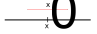
\includegraphics[width=0.5\linewidth]{img/img101}
		\end{center}
	\end{itemize}
\end{frame}

\begin{frame}
	\frametitle{Definisi Deret Taylor}
	\begin{itemize}
		\item Misalkan $ x - x_0 = h $, maka:
		\begin{align*}
			f(x) =& f(x_0) + \frac{h}{1!}f'(x_0) + \frac{h^2}{2!}f''(x_0) + \frac{h^3}{1!}f'''(x_0) \\
			&+ \dots + \frac{h^m}{m!}f^m(x_0) + \dots
		\end{align*}
		\item \textbf{Contoh 1}: Hampiri fungsi $ f(x) = \sin(x) $ ke dalam deret Taylor di sekitar $ x_0 = 1 $.
		\item \textbf{Penyelesaian:}
			\begin{align*}
				f(x) = \sin(x),~ &f'(x) = \cos(x),~f''(x) = -\sin(x) \\
				&f'''(x) = -\cos(x), f^{(4)}(x) = -\cos(x)
			\end{align*}
	\end{itemize}
\end{frame}

\begin{frame}
	\begin{align*}
		\sin(x) =&~ \sin(1) + \frac{(x-1)}{1!}\cos(1) + \frac{(x-1)^2}{2!}(-\sin(1)) \\
		& + \frac{(x-1)^3}{3!}(-\cos(1)) + \frac{(x-1)^4}{4!}\sin(1) + \dots
	\end{align*}

	Misalkan $ x - 1 = h $, maka
	
	\begin{align*}
		\sin(x) =&~ \sin(1) + h\cos(1) + \frac{h^2}{2}(-\sin(1)) + \frac{h^3}{6}(-\cos(1)) \\
		&+ \frac{h^4}{24}\sin(1) + \dots \\
		=&~ 0.8415 + 0.5403h - 0.4208h^2 - 0.0901h^3 + 0.0351h^4 + \dots
	\end{align*}
\end{frame}

\section{Deret Maclaurin}

\begin{frame}
	\frametitle{Deret Maclaurin}
	\begin{itemize}
		\item Kasus khusus: jika $ x_0 = 0$, maka deretnya dinamakan \textbf{Deret Maclaurin}, yang merupakan deret Taylor baku.
		\item \textbf{Contoh 2:} $ \sin(x) $, $ e^x $, $ \cos(x) $ dan $ \ln(x+1) $ masing-masing dalam deret Maclaurin
		\begin{align*}
			\sin(x) =&~ \sin(0) + \frac{(x-0)}{1!}\cos(0) + \frac{(x-0)^2}{2!}(-\sin(0)) \\
			& + \frac{(x-0)^3}{3!}(-\cos(0)) + \frac{(x-0)^4}{4!}\sin(0) + \dots \\
			=&~ x - \frac{x^3}{3!} + \frac{x^5}{5!} - \dots
		\end{align*}
	\end{itemize}
\end{frame}

\begin{frame}
	\begin{itemize}
		\item[]
		\begin{align*}
			e^x =&~ e^{(0)} + \frac{(x-0)}{1!}e^{(0)} + \frac{(x-0)^2}{2!}e^{(0)} + \frac{(x-0)^3}{3!}e^{(0)} \\
			&+ \frac{(x-0)^4}{4!}e^{(0)} \\
			=&~ 1 + x + \frac{x^2}{2!} + \frac{x^3}{3!} + \frac{x^4}{4!} + \dots
		\end{align*}
	\end{itemize}
\end{frame}

\begin{frame}
	\begin{itemize}
		\item[]
		\begin{align*}
			\cos(x) =&~ 1 - \frac{x^2}{2!} + \frac{x^4}{4!} - \frac{x^6}{6!} + \dots
		\end{align*}
	
		\begin{align*}
			\ln(x+1) =&~ \ln(0+1) + \frac{(x-0)}{1!}(0+1)^{-1} + \frac{(x-0)^2}{2!}(-(0+1)^{-2}) \\
			&+ \frac{(x-0)^3}{3!}(2(0+1)^{-3}) + \frac{(x-0)^4}{4!}(-6(0+1)^{-4}) + \dots \\
			=&~ x - \frac{x^2}{2} + \frac{x^3}{3} - \frac{x^4}{4} + \dots
		\end{align*}
	\end{itemize}
\end{frame}

\begin{frame}
	\frametitle{Deret Taylor Terpotong}
	\begin{itemize}
		\item Karena suku-suku deret Taylor tidak berhingga banyaknya, maka -\textit{untuk alasan praktis}- deret Taylor dipotong sampai suku orde tertentu.
		\item Deret Taylor yang dipotong sampai suku orde ke-$ n $ dinamakan \textbf{deret Taylor terpotong} dan dinyatakan oleh:
		\begin{align*}
			f(x) \approx&~f(x_0) + \frac{(x-x_0)}{1!}f'(x_0) + \frac{(x-x_0)^2}{2!}f''(x_0) + \dots \\
			& + \frac{(x-x_0)^n}{n!}f^(n)(x_0) + R_n(x) \\
			R_n(x) =&~ \frac{(x-x_0)^{(n+1)}}{(n+1)!}f^{(n+1)}(c),~~x_0 < c < x
		\end{align*}
		\item $ R_n(x) $ adalah \textbf{Galat/residu/sisa.}
	\end{itemize}
\end{frame}

\begin{frame}
	\frametitle{Deret Maclaurin Terpotong}
	\begin{itemize}
		\item Deret Taylor terpotong di sekitar $ x_0 = 0 $ disebut \textbf{deret Maclaurin terpotong.}
		\item \textbf{Contoh 3:}
		\begin{align*}
			&\sin(x) = x - \frac{x^3}{3!} + \frac{x^5}{5!} + R_5(x);~ R_5(x) = \frac{x^6}{6!}\cos(c) \\
			&e^x = 1 + x + \frac{x^2}{2!} + \frac{x^3}{3!} + \frac{x^4}{4!} + R_4(x);~R_4(x) = \frac{x^5}{5!}e^c \\
			&\cos(x) = 1 - \frac{x^2}{2!} + \frac{x^4}{4!} - \frac{x^6}{6!} + R_6(x);~R_6(x) = \frac{x^7}{7!}\cos(c) \\
			&\ln(x+1) = x - \frac{x^2}{2} + \frac{x^3}{3} - \frac{x^4}{4} + R_4(x);~R_4(x) = \frac{x^5}{5!}(c+1)^{-5}
		\end{align*}
		dimana $ 0 < c < x $.
	\end{itemize}
\end{frame}

\begin{frame}
	\begin{itemize}
		\item \textbf{Contoh 4:} Hitung hampiran nilai $ \cos(0.2) $
		\[ \cos(0.2) \approx 1 - \frac{0.2^2}{2} + \frac{0.2^4}{24} - \frac{0.2^6}{720} = 0.9800667 \]
	\end{itemize}
\end{frame}

\section{Analisis Galat}

\begin{frame}
	\frametitle{Analisis Galat}
	\begin{itemize}
		\item Solusi dengan metode numerik adalah solusi hampiran (aproksimasi).
		\item Hampiran terhadap solusi eksak.
		\item Oleh karena itu, solusi numerik mengandung galat.
		\item \textbf{Galat ($\varepsilon$)}: perbedaan antara solusi hampiran dengan solusi eksak. \[ \varepsilon = a - \hat{a} \]
		\item Galat mutlak: $|\varepsilon| = | a - \hat{a} |$
		\item Galat relatif: $ \varepsilon_R = \frac{\varepsilon}{a} $ atau $\varepsilon_R = \frac{\varepsilon}{a}\times 100\%$
		\item Galat relatif hampiran: $\varepsilon_{RA} = \frac{\varepsilon}{\hat{a}}$
	\end{itemize}
\end{frame}

\begin{frame}
	\begin{itemize}
		\item \textbf{Contoh 5:} Misalkan nilai sejati = 10/3 dan nilai hampiran = 3.333. Hitunglah galat, galat mutlak, galat relatif, dan galat relatif hampiran.\\
		\textbf{Penyelesaian:}\\
		galat = $10/3 - 3.333 = 10/3 - 3333/1000 = 1/3000 = 0.00333...$\\
		galat mutlak = $ |0.000333...| = 0.000333... $\\
		galat relatif = $ (1/3000)/(10/3) = 1/1000 = 0.0001 $\\
		galat relatif hampiran = $ (1/3000)/3.333 = 1/9999 $
	\end{itemize}
\end{frame}

\begin{frame}
	\frametitle{Sumber utama galat}
	\begin{itemize}
		\item Sumber utama galat:
		\begin{enumerate}
			\item Galat pemotongan (\textit{truncation error})
			\item Galat pembulatan (\textit{round-off error})
		\end{enumerate}
		\item \textbf{Galat pemotongan:} galat yang ditimbulkan akibat penggunaan hampiran sebagai pengganti formula eksak\\
		Contoh: hampiran cos(x) dengan deret Maclaurin:\\
		\begin{center}
			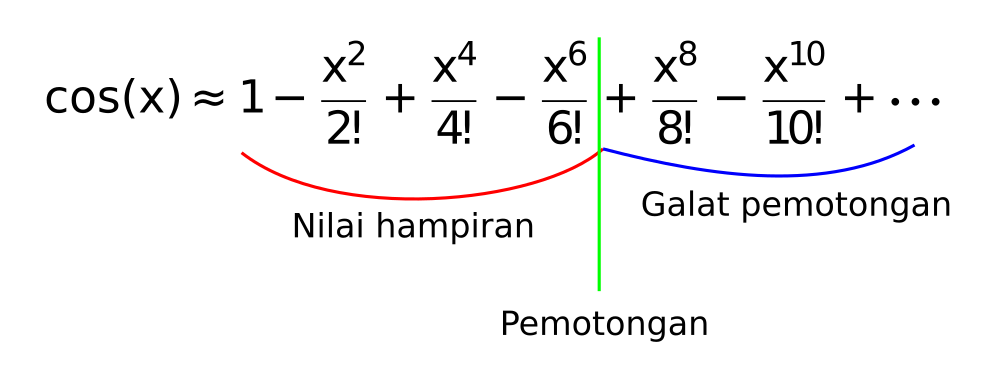
\includegraphics[width=0.6\linewidth]{img/img102.png}
		\end{center}
	\end{itemize}
\end{frame}

\begin{frame}
	\frametitle{Sumber utama galat}
	\begin{itemize}
		\item \textbf{Galat pembulatan:} galat yang timbul akibat keterbatasan komputer dalam merepresentasikan bilangan riil.
		\item \textbf{Contoh 6:} $ 1/6 =  0.1666666666 \dots $ , dalam mesin dengan 6-digit direpresentasikan sebagai 0.166667. Galat pembulatan = 1/6 – 0.166667 = -0.000000333
		\item Contoh dalam sistem biner misalnya $1/10 =  0.00011001100110011001100110011\dots_2 $ direpresentasikan di dalam komputer dalam jumlah bit yang terbatas. 
	\end{itemize}
\end{frame}

\begin{frame}
	\frametitle{Representasi bilangan riil di dalam komputer}
	\begin{itemize}
		\item \textbf{Bilangan titik-tetap (fixed-point):} Setiap bilangan riil disajikan dengan jumlah tempat desimal yang tetap\\
		Contoh: 62.358, 0.013, 1.000.
		\item \textbf{Bilangan titik-kambang (floating-point):} Setiap bilangan riil disajikan dengan jumlah digit berarti yang sudah tetap\\
		Contoh: $0.6238 \times 10^3$ , $0.1714 \times 10^{-13}$
	\end{itemize}
\end{frame}

\begin{frame}
	\frametitle{Angka Bena (Signifikan)}
	\begin{itemize}
		\item Angka bena adalah angka bermakna, angka penting, atau angka yang dapat digunakan dengan pasti.
		\item Contoh:
		\begin{itemize}
			\item[] 43.123 memiliki 5 angka bena (yaitu 4, 3, 1, 2, 3)
			\item[]0.1764 memiliki 4 angka bena (yaitu 1, 7, 6, 4)
			\item[] 0.0000012 memiliki 2 angka bena (yaitu 1, 2)
			\item[] 278.300 memiliki 6 angka bena (yaitu 2, 7, 8, 3, 0, 0)
			\item[] 270.0090 memiliki 7 angka bena (yaitu 2, 7, 0, 0, 0, 9, 0)
			\item[] 0.0090 memiliki 2 angka bena (yaitu 9, 0)
			\item[] 1360, 1.360, 0.001360 semuanya memiliki 4 angka bena
		\end{itemize}
	\end{itemize}
\end{frame}

\begin{frame}
	\frametitle{Angka Bena (Signifikan)}
	\begin{itemize}
		\item Komputer hanya menyimpan sejumlah tertentu angka bena.
		\item Bilangan riil yang jumlah angka benanya melebihi jumlah angka bena komputer akan disimpan dalam sejumlah angka bena komputer itu.
		\item Pengabaian angka bena sisanya itulah yang menimbulkan galat pembulatan
	\end{itemize}
\end{frame}

\begin{frame}
	\frametitle{Galat total}
	\begin{itemize}
		\item \textbf{Galat total:} adalah galat akhir pada solusi numerik merupakan jumlah galat pemotongan dan galat pembulatan.
		\item \textbf{Contoh 7:}
		\begin{center}
			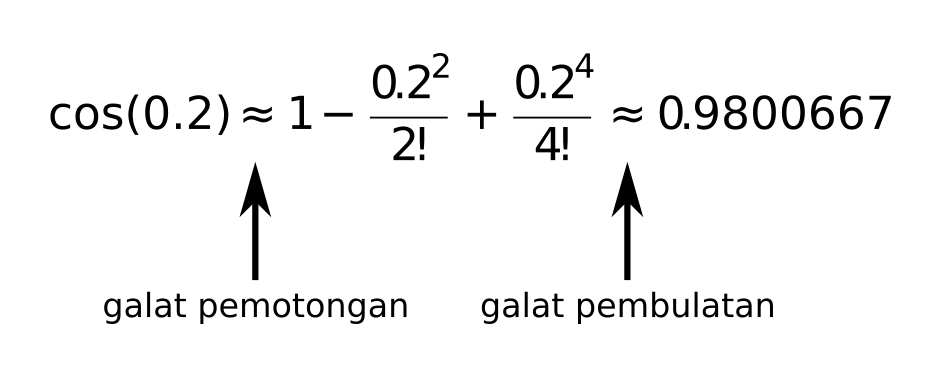
\includegraphics[width=0.6\linewidth]{img/img103.png}
		\end{center}
		\item Pada contoh di atas, galat pemotongan timbul karena kita menghampiri $ \cos(0.2) $ sampai suku orde empat, sedangkan galat pembulatan timbul karena kita membulatkan nilai hampiran ke dalam 7 digit bena.
	\end{itemize}
\end{frame}

\begin{frame}
	\frametitle{Bilangan Titik-Kambang}
	\begin{itemize}
		\item Bilangan riil di dalam komputer umumnya disajikan dalam format bilangan titik-kambang.
		\item Bilangan titik-kambang $ a $ ditulis sebagai
		\[ a = \pm m \times B^p = \pm 0.d_2 d_3 d_4 d_5 d_6 d_2 \dots d_n \times B^p \]
		m = mantisa (riil), $ 0.d_2 d_3 d_4 d_5 d_6 d_2 \dots d_n $ adalah digit mantisa.\\
		B = basis sistem bilangan yang dipakai (2, 8, 10, 16, dsb)\\
		p = pangkat (bilangan bulat), dari $ -P_{min} $ sampai $ +P_{maks} $
		\item contoh $ 245.7654 \rightarrow 0.2457654 \times 10^3 $
	\end{itemize}
\end{frame}

\begin{frame}
	\frametitle{Bilangan Titik-Kambang Ternormalisasi}
	\begin{itemize}
		\item Syarat: digit mantis yang pertama tidak boleh 0
		\item Pada sistem desimal, $ 1 \leq d_1 \leq 9 $ dan $ 0 \leq d_k \leq 9 $,
		sedangkan pada sistem biner, $ d_1 = 1 $ dan $ 0 \leq d_k \leq 1 $.
		\item \textbf{Contoh 8:} 
		\begin{align*}
			0.0563 \times 10{-3} &\rightarrow 0.563 × 10^{-4} \\
			0.00023270 × 10^6 &\rightarrow 0.23270 \times 10^3
		\end{align*}
	\end{itemize}
\end{frame}

\begin{frame}
	\frametitle{Pembulatan pada Bilangan Titik-Kambang}
	\begin{itemize}
		\item Bilangan riil di dalam komputer mempunyai rentang nilai yang terbatas.
		\item Bilangan titik-kambang yang tidak dapat mencocoki satu dari nilai-nilai di dalam rentang nilai yang tersedia, dibulatkan ke salah satu nilai di dalam rentang.
		\item Galat yang timbul akibat penghampiran tersebut diacu sebagai \textbf{galat pembulatan}.
		\item Ada dua teknik pembulatan yang lazim dipakai oleh komputer, yaitu \textbf{pemenggalan} (\textit{chopping}) dan \textbf{pembulatan ke digit terdekat} (\textit{in-rounding}).
	\end{itemize}
\end{frame}

\begin{frame}
	\frametitle{Pemenggalan (chopping)}
	\begin{itemize}
		\item Misalkan $ a = \pm 0.d_1 d_2 d_3 \dots d_nd_{n+1} \dots \times 10^p $\\
		$ fl_{chop}(a) = \pm 0.d_1 d_2 d_3 \dots d_{n-1}d_n \times 10^p $
		\item Contoh: $ \pi = 0.31459265358 \dots \times 10^0 $\\
		$ fl_{chop(\pi)} = 0.3141592 × 100 $ ( 6 digit mantis)\\
		Galat = $ 0.00000065\dots $
	\end{itemize}
\end{frame}

\begin{frame}
	\frametitle{Pembulatan ke digit terdekat (in-rounding)}
	\begin{itemize}
		\item Misalkan $ a = \pm 0.d_1 d_2 d_3 \dots d_nd_{n+1} \dots \times 10^p $\\
		$ fl_{chop}(a) = \pm 0.d_1 d_2 d_3 \dots d_{n-1}d_n \times 10^p $
	\end{itemize}
\end{frame}
% ----------------------------------------------------------------------------
	
\end{document}
